\newpage
\def\thoigian{90}
\de{Đề số 3}{Chương IV. Nguyên hàm – Tích phân}
\begin{center}
	\textbf{PHẦN 1 - CÂU TRẮC NGHIỆM BỐN PHƯƠNG ÁN}
\end{center}
\setcounter{ex}{0}
\Opensolutionfile{ans}[ans/2D4-OTC-TN-Deso3]
\begin{ex}%[2D4N1-1]%[Dự án D đợt 4 - Nguyễn Hoàng Anh]%[Đề ôn tập Chương IV - Khối 12 - Đề số 3]
	Cho $y=f(x)$ và $y=g(x)$ là các hàm số xác định và liên tục trên khoảng $(a;b)$. Khẳng định nào sau đây là $\textbf{sai}$?
	\choice
	{$\displaystyle \int{\left[f(x)+g(x)\right]}\mathrm{\,d}x = \displaystyle \int{f(x)}\mathrm{\,d}x +\displaystyle \int{g(x)}\mathrm{\,d}x$}
	{$\displaystyle \int{\left[f(x)-g(x)\right]}\mathrm{\,d}x = \displaystyle \int{f(x)}\mathrm{\,d}x -\displaystyle \int{g(x)}\mathrm{\,d}x$}
	{\True $\displaystyle \int{\left[f(x) \cdot g(x)\right]}\mathrm{\,d}x = \displaystyle \int{f(x)}\mathrm{\,d}x \cdot \displaystyle \int{g(x)}\mathrm{\,d}x$}
	{$\displaystyle \int{kf(x)}\mathrm{\,d}x = k\displaystyle \int{f(x)}\mathrm{d}x$ (với $\forall k \neq 0$)}
	\loigiai{
		Không có tính chất $\displaystyle \int{\left[f(x) \cdot g(x)\right]}\mathrm{\,d}x = \displaystyle \int{f(x)}\mathrm{\,d}x \cdot \displaystyle \int{g(x)}\mathrm{\,d}x$.
		}
\end{ex}
\begin{ex}%[2D4N1-1]%[Dự án D đợt 4 - Nguyễn Hoàng Anh]%[Đề ôn tập Chương IV - Khối 12 - Đề số 3]
	Khẳng định nào sau đây là $\textbf{sai}$?
	\choice
	{$\displaystyle \int x\mathrm{\,d}x = \dfrac{1}{2} x^2 + C$}
	{$\displaystyle \int e^{x}\mathrm{\,d}x = e^{x} + C$}
	{\True $\displaystyle \int \cos x\mathrm{\,d}x = -\sin x + C$}
	{$\displaystyle \int \dfrac{1}{x}\mathrm{\,d}x = \ln |x| + C$}
	\loigiai{
		Ta có $\displaystyle \int \cos x\mathrm{\,d}x = \sin x + C$.}
\end{ex}
\begin{ex}%[2D4N1-2]%[Dự án D đợt 4 - Nguyễn Hoàng Anh]%[Đề ôn tập Chương IV - Khối 12 - Đề số 3]
	Nguyên hàm của hàm số $f(x)=\dfrac{1}{\sqrt{x}}$ trên khoảng $(0; +\infty)$ là
	\choice
	{$\sqrt{x}+C$}
	{\True $2\sqrt{x}+C$}
	{$\dfrac{\sqrt{x}}{2}+C$}
	{$\dfrac{2}{\sqrt{x}}+C$}
	\loigiai{
	Ta có $\displaystyle\int f(x)\mathrm{\,d}x=\displaystyle\int \dfrac{1}{\sqrt{x}}\mathrm{\,d}x=2\displaystyle\int \dfrac{1}{2\sqrt{x}}\mathrm{\,d}x=2\sqrt{x}+C$.
	}
\end{ex}
\begin{ex}%[2D4N1-3]%[Dự án D đợt 4 - Nguyễn Hoàng Anh]%[Đề ôn tập Chương IV - Khối 12 - Đề số 3]
	Nguyên hàm của hàm số $f(x)=2x+\sin x$ là
	\choice
	{$x^2+\cos x+C$}
	{\True $x^2-\cos x+C$}
	{$2-\cos x+C$}
	{$2+\cos x+C$}
	\loigiai{
	Ta có $\displaystyle\int f(x)\mathrm{\,d}x=\displaystyle\int (2x+\sin x)\mathrm{\,d}x=x^2-\cos x+C$.
	}
\end{ex}
\begin{ex}%[2D4N2-1]%[Dự án D đợt 4 - Nguyễn Hoàng Anh]%[Đề ôn tập Chương IV - Khối 12 - Đề số 3]
	Gọi $F\left(x\right)$ là một nguyên hàm của hàm số $f(x)$ trên đoạn $\left[a;b\right]$. Khẳng định nào sau đây đúng?
	\choice
	{$\displaystyle\int\limits_{a}^{b}f(x)\mathrm{\,d}x=F(a)-F(b)$}
	{$\displaystyle\int\limits_{a}^{b}f(x)\mathrm{\,d}x=F(a)+F(b)$}
	{\True $\displaystyle\int\limits_{a}^{b}f(x)\mathrm{\,d}x=F(b)-F(a)$}
	{$\displaystyle\int\limits_{a}^{b}f(x)\mathrm{\,d}x=F(a)\cdot F(b)$}
	\loigiai{
	Theo định nghĩa tích phân ta có:
	\begin{center}
		$\displaystyle\int\limits_{a}^{b}f(x)\mathrm{\,d}x=F(x)\biggl |_a^b=F(b)-F(a)$.
	\end{center}
	}
\end{ex}
\begin{ex}%[2D4N2-1]%[Dự án D đợt 4 - Nguyễn Hoàng Anh]%[Đề ôn tập Chương IV - Khối 12 - Đề số 3]
Cho hàm số $y=f(x)$ liên tục trên $\mathbb{R}$ và thỏa mãn $\displaystyle\int\limits_{1}^{3}f(x)\mathrm{\,d}x=5$ và $\displaystyle\int\limits_{3}^{7}f(x)\mathrm{\,d}x=9$. Giá trị của $\displaystyle\int\limits_{1}^{7}f(x)\mathrm{\,d}x$ bằng  
\choice
{\True $14$ }
{$45$}
{$4$}
{$-4$}
\loigiai{
	Ta có $\displaystyle\int\limits_{1}^{7}f(x)\mathrm{\,d}x=\displaystyle\int\limits_{1}^{3}f(x)\mathrm{\,d}x+\displaystyle\int\limits_{3}^{7}f(x)\mathrm{\,d}x=5+9=14$.
	
}
\end{ex}
\begin{ex}%[2D4H2-1]%[Dự án D đợt 4 - Nguyễn Hoàng Anh]%[Đề ôn tập Chương IV - Khối 12 - Đề số 3]
	Nếu $\displaystyle\int\limits_{0}^{2}f(x) \mathrm{\,d}x=4$ thì $\displaystyle\int\limits_{0}^{2}\left[\dfrac{1}{2}f(x)-2\right] \mathrm{d}x$ bằng
	\choice
	{$0$}
	{$6$}
	{$8$}
	{\True$-2$}
	\loigiai{
		Ta có $\displaystyle\int\limits_{0}^{2}\left[\dfrac{1}{2}f(x)-2\right] \mathrm{\,d}x=\dfrac{1}{2}\displaystyle\int\limits_{0}^{2}f(x)\mathrm{\,d}x-\displaystyle\int\limits_{0}^{2}2 \mathrm{\,d}x=\dfrac{1}{2}\cdot 4-4=-2$.
	}
\end{ex}
\begin{ex}%[2D4H2-1]%[Dự án D đợt 4 - Nguyễn Hoàng Anh]%[Đề ôn tập Chương IV - Khối 12 - Đề số 3]
	Cho hàm số $f(x)$ có đạo hàm liên tục trên đoạn $[2; 4]$, biết $f(4)=6$ và $\displaystyle\int\limits_2^4f'(x) \mathrm{\,d}x=4$. Giá trị của $f(2)$ bằng
	\choice
	{\True $2$}
	{$-2$}
	{$10$}
	{$24$}
	\loigiai{
		Ta có $\displaystyle\int\limits_2^4f'(x) \mathrm{\,d}x=f(x) \biggl |_2^4=f(4)-f(2)$.\\
		Mà theo giả thiết $\displaystyle\int\limits_2^4f'(x) \mathrm{\,d}x=4 \Leftrightarrow f(4)-f(2)=4 \Rightarrow f(2)=f(4)-4=2$.
	}
\end{ex}
\begin{ex}%[2D4N3-3]%[Dự án D đợt 4 - Nguyễn Hoàng Anh]%[Đề ôn tập Chương IV - Khối 12 - Đề số 3]
	Cho hàm số $y=f\left( x \right)$ liên tục trên đoạn $\left[ a;b \right]$. Gọi $D$ là hình phẳng giới hạn bởi đồ thị hàm số $y=f\left( x \right)$, trục hoành và hai đường thẳng $x=a$, $x=b$ $(a<b)$. Thể tích khối tròn xoay được tạo thành khi quay $D$ quanh trục hoành là
	\choice
	{\True $V=\pi \displaystyle\int\limits_a^b{{[f\left( x \right)]}^2} \mathrm{d} x$}
	{ $V=2\pi \displaystyle\int\limits_a^b{{[f\left( x \right)]}^2}\mathrm{d} x$}
	{ $V={{\pi }^2}\displaystyle\int\limits_a^b{{[f\left( x \right)]}^2}\mathrm{d} x$}
	{ $V={{\pi }^2}\displaystyle\int\limits_a^bf\left( x \right)\mathrm{d} x$}
	\loigiai{
		Thể tích khối tròn xoay là $V=\pi \displaystyle\int\limits_a^b{{[f\left( x \right)]}^2}\mathrm{d} x$.
	}
\end{ex}
\begin{ex}%[2D4H3-3]%[Dự án D đợt 4 - Nguyễn Hoàng Anh]%[Đề ôn tập Chương IV - Khối 12 - Đề số 3]
	Cho hình phẳng $\left( H \right)$ giới hạn bởi đồ thị $y=2x-x^2$ và trục hoành. Thể tích vật thể tròn xoay sinh ra khi cho $\left( H \right)$ quay quanh trục hoành bằng
	\choice
	{$\dfrac{16}{15}$}
	{$\dfrac{4}{3}$}
	{\True $\dfrac{16\pi}{15}$}
	{$\dfrac{4\pi}{3}$}
	\loigiai{
		Phương trình hoành độ giao điểm của đồ thị $y=2x-x^2$ và trục hoành là
		$$2x-x^2=0\Leftrightarrow \hoac{& x=0 \\ & x=2.}$$
		Thể tích vật thể tròn xoay sinh ra khi cho $\left( H \right)$ quay quanh trục hoành là
		$$V=\pi \displaystyle\int\limits_0^2 \left( 2x-x^2 \right)^2 \mathrm{\,d}x=\dfrac{16\pi}{15}.$$
	}
\end{ex}
\begin{ex}%%[2D3N3-1]%[Dự án D đợt 4 - Nguyễn Hoàng Anh]%[Đề ôn tập Chương IV - Khối 12 - Đề số 3]
	Diện tích hình phẳng giới hạn bởi các đường $y=x^2$ và $y=x+2$ là
	\choice
	{$S=9$}
	{$S=\dfrac{9}{4}$}
	{\True $S=\dfrac{9}{2}$}
	{$S=\dfrac{8}{9}$}
	\loigiai{Phương trình hoành độ giao điểm của đồ thị hàm số $y=x^2$ và đường thẳng $y=x+2$ là
		\[x^2=x+2\Leftrightarrow x^2-x-2=0\Leftrightarrow\hoac{&x=-1\\&x=2.}\]
		Diện tích hình phẳng giới hạn bới các đường $y=x^2$ và $y=x+2$ là
		\[S=\displaystyle\int\limits_{-1}^2\left|x^2-x-2\right|\mathrm{\,d}x=-\displaystyle\int\limits_{-1}^2\left(x^2-x-2\right)\mathrm{\,d}x=-\left(\dfrac{x^3}{3}-\dfrac{x^2}{2}-2x\right)\Bigg|_{-1}^2=\dfrac{9}{2}.\]}
\end{ex}
\begin{ex}%[2D4N2-1]%[Dự án D đợt 4 - Nguyễn Hoàng Anh]%[Đề ôn tập Chương IV - Khối 12 - Đề số 3]
	\immini[thm]{Diện tích hình phẳng gạch sọc trong hình vẽ bên dưới bằng
		\choice
		{\True $\displaystyle\int \limits_1^3 (2^x-2)\mathrm{d}x$}
		{$\displaystyle\int \limits_1^3 (2^x+2)\mathrm{d}x$}
		{$\displaystyle\int \limits_1^3 (2-2^x)\mathrm{d}x$}
		{$\displaystyle\int \limits_1^3 2^x\mathrm{d}x$}}{
		\begin{tikzpicture}[scale=0.6, font=\footnotesize, line join=round, line cap=round, >=stealth]
			\def \xmin{-3.1}\def \xmax{4.1}\def \ymin{-1}\def \ymax{9} 
			\draw[->] (\xmin,0)--(\xmax,0) node[shift=(-110:0.2)] {$x$};
			\draw[->] (0,\ymin)--(0,\ymax) node[shift=(-150:0.2)] {$y$};
			\fill (0,0) circle(1pt) node[shift=(-135:0.25)]{$O$};
			%Vẽ các điểm trên trục Ox
			\foreach \x/\g in {1/-90,3/-90}
			\fill (\x,0) circle(1pt) node[shift=(\g:0.2)]{$\x$};
			%Vẽ các điểm trên trục Oy
			\foreach \y/\g in {2/180,8/180}
			\fill (0,\y) circle(1pt) node[shift=(\g:0.2)]{$\y$};
			%Vẽ các điểm gióng
			\foreach \x/\y in {3/2}
			{\draw[dashed,thin] (\x,0)--(\x,\y)--(0,\y);
				\fill (\x,\y) circle(1pt);};
			\node at (2, 5) [above, rotate=38] {$y = 2^{x}$};
			\clip (\xmin,\ymin) rectangle (\xmax,\ymax); 
			\draw[smooth,samples=100,domain=\xmin:\xmax] plot (\x,{2^(\x)});
			\fill[pattern=north east lines] (1,2) plot[domain=1:3](\x,{2^(\x)})--(3,8)--(3,2);
			\draw [dashed](1,2)--(1,0) (0,8)--(3,8)--(3,0);
		\end{tikzpicture}
	}
	\loigiai{
		Hình phẳng gạch sọc trong hình vẽ được giới hạn bởi các đường $y=2^x$, $y=2$, $x=1$ và $x=3$.\\
		Do đó diện tích hình phẳng gạch sọc trong hình vẽ bằng $\displaystyle\int \limits_1^3 |2^x-2|\mathrm{d}x=\displaystyle\int \limits_1^3 (2^x-2)\mathrm{d}x$.}
\end{ex}

\Closesolutionfile{ans}
\begin{center}
	\textbf{PHẦN 2 - CÂU TRẮC NGHIỆM ĐÚNG SAI}
\end{center}
\setcounter{ex}{0}
\Opensolutionfile{ans}[ans/2D4-OTC-DS-Deso3]
\begin{ex}%%[2D4H2-1]%[2D4V2-1]%[Dự án D đợt 4 - Nguyễn Hoàng Anh]%[Đề ôn tập Chương IV - Khối 12 - Đề số 3]
	Cho hàm số bậc ba $f(x)$ có đồ thị nhận gốc tọa độ $O$ làm tâm đối xứng. Gọi $F(x)$ là nguyên hàm của hàm số $f(x)$ trên $\mathbb{R}$ thỏa mãn $F(0)=2$. Biết rằng $\displaystyle\int\limits_{0}^{3} f(x)\mathrm{\,d}x=5$.
	\choiceTF
	{\True $F(3)=7$}
	{\True $\displaystyle\int\limits_{0}^{3} \left[2f(x)-3\right]\mathrm{\,d}x=1$}
	{$F(-3)=-7$}
	{Nếu $G(x)$ là một nguyên hàm khác của $f(x)$ trên $\mathbb{R}$ và thỏa mãn $F(3)-G(0)=10$ thì $G(x)=F(x)+4$ với mọi số thực $x$}
	\loigiai{
	\begin{itemchoice}
	\itemch Ta có $\displaystyle\int\limits_{0}^{3} f(x)\mathrm{\,d}x=5\Leftrightarrow F(3)-F(0)=5\Leftrightarrow F(3)-2=5 \Leftrightarrow F(3)=7$.
	\itemch	Ta có $\displaystyle\int\limits_{0}^{3} \left[2f(x)-3\right]\mathrm{\,d}x=2\displaystyle\int\limits_{0}^{3} f(x)\mathrm{\,d}x-\displaystyle\int\limits_{0}^{3} 3\mathrm{\,d}x=2\cdot 5 - 9=1$.
	\itemch Do $f(x)$ là hàm số bậc ba có đồ thị nhận gốc tọa độ $O$ là tâm đối xứng nên \begin{center}
	$\displaystyle\int\limits_{-3}^{0} f(x)\mathrm{\,d}x=-\displaystyle\int\limits_{0}^{3} f(x)\mathrm{\,d}x=-5$.
	\end{center}
	Suy ra $F(0)-F(-3)=-5\Leftrightarrow 2-F(-3)=-5 \Leftrightarrow F(-3)=7$.
	\itemch Ta có $F(3)-G(0)=10 \Leftrightarrow 7-G(0)=10 \Leftrightarrow G(0)=-3$.\\
	Do $G(x)$ cũng là một nguyên hàm của hàm số $f(x)$ nên tồn tại một hằng số $C$ để $G(x)=F(x)+C$ với mọi số thực $x$.\\
	Suy ra $G(0)=F(0)+C \Leftrightarrow -3=2+C \Leftrightarrow C=-5$.\\
	Do đó $G(x)=F(x)-5$.\\
	\end{itemchoice}
	}
\end{ex}
\begin{ex}%[2D4N3-1]%%[2D4V3-1][Dự án D đợt 4 - Nguyễn Hoàng Anh]%[Đề ôn tập Chương IV - Khối 12 - Đề số 3]
	Cho hàm số bậc hai $y=f(x)$ có đồ thị là parabol $(P)$ và đường thẳng $d \colon y=g(x)$. Biết $d$ cắt $(P)$ tại hai điểm có tọa độ là $(3;8)$ và $(7;0)$. Hình phẳng $(H)$ giới hạn bởi parabol $(P)$ và đường thẳng $d$ có diện tích bằng $\dfrac{32}{3}$.
	\begin{center}
		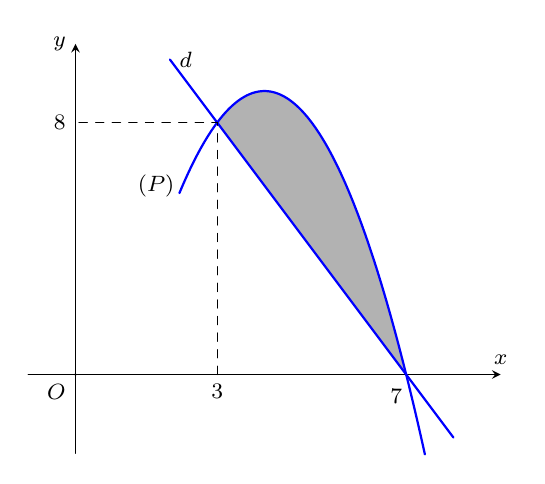
\begin{tikzpicture}[scale=0.4, font=\footnotesize, line join=round, line cap=round, >=stealth,xscale=1.5]
			% Trục tọa độ
			\draw[->] (-1,0) -- (9,0) node[above] {$x$};
			\draw[->] (0,-2.5) -- (0,10.5) node[left] {$y$};
			\fill (0,0) circle (1pt) node[below left]{$O$};
			\begin{scope}
				\clip (3,0) rectangle (7,9); % Giới hạn vùng tô giữa
				\fill[gray!60] plot[domain=3:7, samples=100] (\x,{(-1)*(\x)^2+8*(\x)-7})
				-- plot[domain=7:3, samples=100] (\x,{-2*(\x)+14}) -- cycle;
			\end{scope}
			\draw[blue,thick,samples=300] plot[domain=2.2:7.4](\x,{(-1)*(\x)^2+8*(\x)-7});
			\draw[blue,thick,samples=300] plot[domain=2:8](\x,{-2*(\x)+14});
			\draw[dashed] (3,0)node[below]{$3$}--(3,8)--(0,8)node[left]{$8$};
			%	\draw[dashed] (6,0)--(6,12)--(0,12)node[left]{$12$};
			\node at (7,0) [shift=(245:0.3)]{$7$};
			\node at (2.3,6) [left]{$(P)$};
			\node at (2,10) [right]{$d$};
		\end{tikzpicture}
	\end{center}
	\choiceTF 
	{$\displaystyle\int\limits_{3}^{7}[g(x)-f(x)]\mathrm{\,d}x=\dfrac{32}{3}$}
	{\True $\displaystyle\int\limits_{3}^{7}f(x)\mathrm{\,d}x=\dfrac{80}{3}$}
	{\True $\displaystyle\int\limits_{3}^{7}\left[2f^{\prime}(x)+1\right]\mathrm{\,d}x=-12$}
	{\True $f(10)=-27$}
	\loigiai{
			\begin{center}
			\begin{tikzpicture}[scale=0.4, font=\footnotesize, line join=round, line cap=round, >=stealth,xscale=1.5]
				% Trục tọa độ
				\draw[->] (-1,0) -- (9,0) node[above] {$x$};
				\draw[->] (0,-2.5) -- (0,10.5) node[left] {$y$};
				\fill (0,0) circle (1pt) node[below left]{$O$};
				\begin{scope}
					\clip (3,0) rectangle (7,9); % Giới hạn vùng tô giữa
					\fill[gray!60] plot[domain=3:7, samples=100] (\x,{(-1)*(\x)^2+8*(\x)-7})
					-- plot[domain=7:3, samples=100] (\x,{-2*(\x)+14}) -- cycle;
				\end{scope}
				\begin{scope}
					\clip (3,0) rectangle (7,9);
					\fill[pattern=north east lines] 
					plot[domain=3:7, samples=100] (\x,{-2*(\x)+14})
					-- (7,0) -- (3,0) -- cycle;
				\end{scope}
				\draw[blue,thick,samples=300] plot[domain=2.2:7.4](\x,{(-1)*(\x)^2+8*(\x)-7});
				\draw[blue,thick,samples=300] plot[domain=2:8](\x,{-2*(\x)+14});
				\draw[dashed] (3,0)node[below]{$3$}--(3,8)--(0,8)node[left]{$8$};
				%	\draw[dashed] (6,0)--(6,12)--(0,12)node[left]{$12$};
				\node at (7,0) [shift=(245:0.3)]{$7$};
				\node at (2.3,6) [left]{$(P)$};
				\node at (2,10) [right]{$d$};
			\end{tikzpicture}
		\end{center}
	\begin{itemchoice}
	\itemch Dựa vào đồ thị hai hàm số, ta thấy $f(x)>g(x)$ với $\forall x \in (3;7)$.\\	
	Do đó $S(H)=\displaystyle\int\limits_{3}^{7}|f(x)-g(x)|\mathrm{\,d}x=\displaystyle\int\limits_{3}^{7}\left(f(x)-g(x)\right)\mathrm{\,d}x$.\\
	Theo giả thiết $S_{(H)}=\dfrac{32}{3}$, suy ra $\displaystyle\int\limits_{3}^{7}\left(f(x)-g(x)\right)\mathrm{\,d}x=\dfrac{32}{3}$.\\
	Do đó $\displaystyle\int\limits_{3}^{7}[g(x)-f(x)]\mathrm{\,d}x=-\dfrac{32}{3}$
	\itemch Gọi $S'$ là diện tích hình phẳng giới hạn bởi đường thẳng $d$, trục hoành và đường thẳng $x=3$ (phần gạch sọc trên hình vẽ).\\
	Ta có $S'=\dfrac{1}{2}\cdot 8\cdot 4=16$.\\
	Mặt khác $\displaystyle\int\limits_{3}^{7}f(x)\mathrm{\,d}x$ là diện tích của hình phẳng giới hạn bởi parabol $y=f(x)$, trục hoành, đường thẳng $x=3$.\\
	Suy ra $\displaystyle\int\limits_{3}^{7}f(x)\mathrm{\,d}x=S+S'=\dfrac{32}{3}+16=\dfrac{80}{3}$.
	\itemch Ta có $\displaystyle\int\limits_{3}^{7}\left[2f^{\prime}(x)+1\right]\mathrm{\,d}x=\left(2f(x)+x\right)\biggl |_3^7=2(f(7)-f(3))+4=2(0-8)+4=-12$.
	\itemch Giả sử $y=f(x)=ax^2+bx+c$ với $a \neq 0$.\\
	Parabol $y=f(x)$ đi qua hai điểm $(3;8)$ và $(7;0)$ nên $\heva{&9a+3b+c=8 \quad (1)\\&49a+7b+c=0 \quad (2).}$\\
	Mặt khác
	\begin{eqnarray*} 
		&&\displaystyle\int\limits_{3}^{7}f(x)\mathrm{\,d}x=\dfrac{80}{3}\\
		&\Leftrightarrow& \displaystyle\int\limits_{3}^{7} \left(ax^2+bx+c\right)\mathrm{\,d}x=\dfrac{80}{3}\\
		&\Leftrightarrow& \left(\dfrac{ax^3}{3}+\dfrac{bx^2}{2}+cx\right)\biggl |_3^7=\dfrac{80}{3}\\
		&\Leftrightarrow& \dfrac{316}{3}a+20b+4c=\dfrac{80}{3} \quad (3).  
	\end{eqnarray*}
   Từ (1), (2), (3) ta có hệ phương trình $\heva{&9a+3b+c=8\\&49a+7b+c=0\\&\dfrac{316}{3}a+20b+4c=\dfrac{80}{3}}\Leftrightarrow \heva{&a=-1\\&b=8\\&c=-7.}$\\
	Suy ra $f(x)=-x^2+8x-7$.\\
	Do đó $f(10)=-10^2+8\cdot 10-7=-27$.
	\end{itemchoice}
	
	}  	
\end{ex}
\Closesolutionfile{ans}
\begin{center}
	\textbf{PHẦN 3 - CÂU TRẮC NGHIỆM TRẢ LỜI NGẮN}
\end{center}
\setcounter{ex}{0}
\Opensolutionfile{ans}[ans/2D4-OTC-TLN-Deso3]
\begin{ex}%[2D4H2-1]%[Dự án D đợt 4 - Nguyễn Hoàng Anh]%[Đề ôn tập Chương IV - Khối 12 - Đề số 3]
	Cho hàm số $f(x)=\heva{&x^2+x \quad &\text{khi} \quad x 
		\leq 1,\\&\dfrac{1}{x} +1 \quad &\text{khi} \quad x > 1.}$\\
	Biết rằng $\displaystyle\int\limits_{-1}^{2}f(x)\mathrm{\,d}x=\dfrac{a}{b}+\ln c$, ($a, b, c \in \mathbb{Z}$, $\dfrac{a}{b}$ là phân số tối giản). Tính $abc$.
	\shortans[0]{$30$}
	\loigiai{
	Tập xác định của hàm số là $\mathscr{D}=\mathbb{R}$.\\
	Dễ thấy hàm số liên tục trên các khoảng $(-\infty;1)$ và $(1;+\infty)$.\\
	Mặt khác $\displaystyle\lim\limits_{x \to 1^{-}}f(x)=\displaystyle\lim\limits_{x \to 1^{-}}(x^2+x)=2$, $\displaystyle\lim\limits_{x \to 1^{+}}f(x)=\displaystyle\lim\limits_{x \to 1^{+}}\left(\dfrac{1}{x} +1\right)=2$.\\
	Suy ra hàm số đã cho liên tục trên $\mathbb{R}$.\\
	Ta có $\displaystyle\int\limits_{-1}^{2}f(x)\mathrm{\,d}x=\displaystyle\int\limits_{-1}^{1}f(x)\mathrm{\,d}x+\displaystyle\int\limits_{1}^{2}f(x)\mathrm{\,d}x=\displaystyle\int\limits_{-1}^{1}\left(x^2+x\right)\mathrm{\,d}x+\displaystyle\int\limits_{1}^{2}\left(\dfrac{1}{x} +1\right)\mathrm{\,d}x=\dfrac{5}{3}+\ln 2$.\\
	Suy ra $a=5$, $b=3$, $c=2$.\\
	Do đó $abc=5 \cdot 3 \cdot 2 =30$.
	
	}
\end{ex}
\begin{ex}%[2D4H2-1]%[Dự án D đợt 4 - Nguyễn Hoàng Anh]%[Đề ôn tập Chương IV - Khối 12 - Đề số 3]
	Cho $f(x)=x^2\ln x$. Biết rằng $\displaystyle\int\limits_{1}^{3}\left(f^{\prime}(x)+3^x+\dfrac{2}{x}\right)\mathrm{\,d}x=a\ln b +\dfrac{c}{\ln b}$ (với $a$, $b$, $c$ là các số nguyên dương, $b<5$), hãy tính $a+b+c$.
	\shortans[0]{$38$}
	\loigiai{
		Ta có $\displaystyle\int\limits_{1}^{3}\left(f^{\prime}(x)+3^x+\dfrac{2}{x}\right)\mathrm{\,d}x=f(x)\biggl|_1^3+\left(\dfrac{3^x}{\ln 3}+2\ln x\right)\biggl |_1^3=x^2\ln x\biggl|_1^3+\left(\dfrac{3^x}{\ln 3}+2\ln x\right)\biggl |_1^3$.\\
		Suy ra $\displaystyle\int\limits_{1}^{3}\left(f^{\prime}(x)+3^x+\dfrac{2}{x}\right)\mathrm{\,d}x=11\ln 3+\dfrac{24}{\ln 3}$.\\
		Mà theo giả thiết $\displaystyle\int\limits_{1}^{3}\left(f^{\prime}(x)+3^x+\dfrac{2}{x}\right)\mathrm{\,d}x=a\ln b +\dfrac{c}{\ln b}$ (với $a$, $b$, $c$ là các số nguyên dương, $b<5$), suy ra $a=11$, $b=3$ và $c=11$.\\
		Do đó $a+b+c=38$.
		
	}
\end{ex}
\begin{ex}%[2D4V3-2]%[Dự án D đợt 4 - Nguyễn Hoàng Anh]%[Đề ôn tập Chương IV - Khối 12 - Đề số 3]
	\immini{
		Mảnh vườn nhà ông An có dạng hình elip với bốn đỉnh $A_1$, $A_2$, $B_1$, $B_2$ như hình vẽ bên. Ông dùng hai đường Parabol có đỉnh là tâm đối xứng của elip cắt elip tại $4$ điểm $M$, $N$, $P$, $Q$ như hình vẽ sao cho tứ giác $MNPQ$ là hình chữ nhật có $MN=4$ để chia vườn như sau: phần tô đậm thì dùng trồng hoa và phần còn lại để trồng rau. Biết chi phí trồng hoa là $600$ nghìn đồng/m$^2$ và chi phí trồng rau là $50$ nghìn đồng/m$^2$. Hỏi số tiền phải chi bằng bao nhiêu triệu đồng, biết $A_1A_2=8$ m, $B_1B_2=4$ m. (kết quả làm tròn đến hàng phần chục).
	}{
		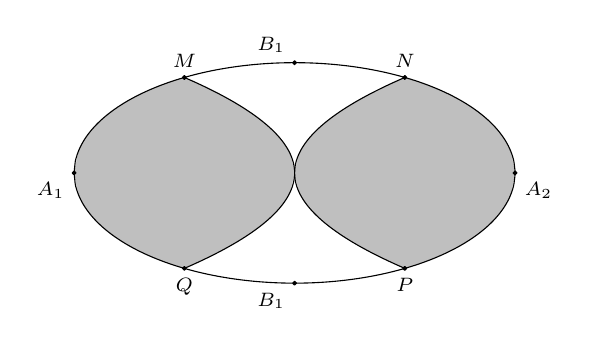
\begin{tikzpicture}[scale=0.7, line join=round, line cap=round, >=stealth,font=\scriptsize]
			\tikzset{every node/.style={scale=1}}
			%			\def\xmin{-5}\def\xmax{5}\def\ymin{-2.5}\def\ymax{4}
			%			\draw[->] (\xmin-0.2,0)--(\xmax+0.2,0) node[below]{$x$};
			%			\draw[->] (0,\ymin-0.2)--(0,\ymax+0.2) node[right]{$y$};
			%			\draw (0,0) node[below left]{$O$};
			%				\foreach \x in {}\draw (\x,0.1)--(\x,-0.1) node[below]{$\x$};
			%				\foreach \y in {}\draw (0.1,\y)--(-0.1,\y) node[left]{$\y$};
			%				\clip (\xmin,\ymin) rectangle (\xmax,\ymax);
			\fill [gray!50, smooth] (-4,0)--plot[domain=-4:-2](\x,{2*sqrt(1-0.0625*(\x)^2)})--plot[domain=-2:0](\x,{sqrt(1.5*(-\x))})--plot[domain=0:-2](\x,{-sqrt(1.5*(-\x))})--plot[domain=-2:-4](\x,{-2*sqrt(1-0.0625*(\x)^2)})--cycle
			;
			\fill [gray!50, smooth] (4,0)--plot[domain=4:2](\x,{2*sqrt(1-0.0625*(\x)^2)})--plot[domain=2:0](\x,{sqrt(1.5*(\x))})--plot[domain=0:2](\x,{sqrt(1.5*(\x))})--plot[domain=2:4](\x,{-2*sqrt(1-0.0625*(\x)^2)})--cycle
			;
			\fill [gray!50, smooth] (0,0)--plot[domain=0:2](\x,{sqrt(1.5*(\x))})--plot[domain=2:4](\x,{2*sqrt(1-0.0625*(\x)^2)})--plot[domain=4:2](\x,{2*sqrt(1-0.0625*(\x)^2)})--plot[domain=2:0](\x,{-sqrt(1.5*(\x))})--cycle
			;
			%Vẽ Elip
			\draw[smooth,samples=200,domain=0: 4] plot (\x,{2*sqrt(1-0.0625*(\x)^2)});
			\draw[smooth,samples=200,domain=0: 4] plot (\x,{-2*sqrt(1-0.0625*(\x)^2)});
			\draw[smooth,samples=200,domain=-4: 0] plot (\x,{2*sqrt(1-0.0625*(\x)^2)});
			\draw[smooth,samples=200,domain=-4: 0] plot (\x,{-2*sqrt(1-0.0625*(\x)^2)});
			%Vẽ Parabol
			\draw[smooth,samples=200,domain=0: 2] plot (\x,{sqrt(1.5*(\x))});
			\draw[smooth,samples=200,domain=0: 2] plot (\x,{-sqrt(1.5*(\x))});
			\draw[smooth,samples=200,domain=-2: 0] plot (\x,{sqrt(1.5*(-\x))});
			\draw[smooth,samples=200,domain=-2: 0] plot (\x,{-sqrt(1.5*(-\x))});
			%Vẽ các đỉnh
			\draw [fill=black] (-4,0)node[below left]{$A_1$}circle(1pt) (4,0)node[below right]{$A_2$}circle(1pt) (0,-2)node[below left]{$B_1$}circle(1pt) (0,2)node[above left]{$B_1$}circle(1pt) (-2,1.732)node[above]{$M$}circle(1pt) (2,1.732)node[above]{$N$}circle(1pt) (2,-1.732)node[below]{$P$}circle(1pt) (-2,-1.732)node[below]{$Q$}circle(1pt) ;
		\end{tikzpicture}
	}
	\par
	\shortans[]{$11{,}7$}
	\loigiai{
		\begin{center}
			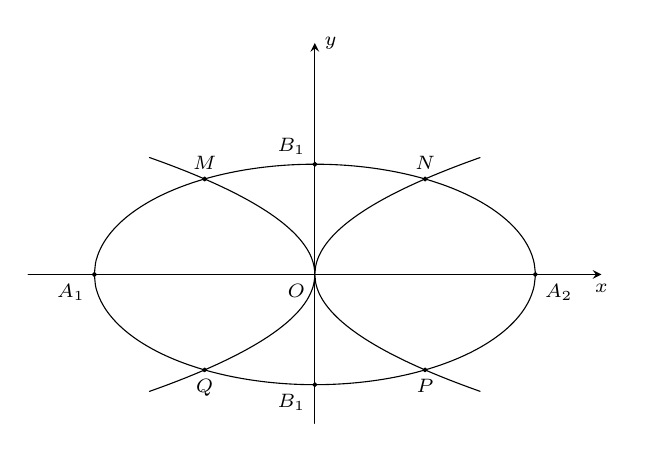
\begin{tikzpicture}[scale=0.7, line join=round, line cap=round, >=stealth,font=\scriptsize]
				\tikzset{every node/.style={scale=1}}
				\def\xmin{-5}\def\xmax{5}\def\ymin{-2.5}\def\ymax{4}
				\draw[->] (\xmin-0.2,0)--(\xmax+0.2,0) node[below]{$x$};
				\draw[->] (0,\ymin-0.2)--(0,\ymax+0.2) node[right]{$y$};
				\draw (0,0) node[below left]{$O$};
				%				\foreach \x in {}\draw (\x,0.1)--(\x,-0.1) node[below]{$\x$};
				%				\foreach \y in {}\draw (0.1,\y)--(-0.1,\y) node[left]{$\y$};
				%				\clip (\xmin,\ymin) rectangle (\xmax,\ymax);
				%Vẽ Elip
				\draw[smooth,samples=200,domain=0: 4] plot (\x,{2*sqrt(1-0.0625*(\x)^2)});
				\draw[smooth,samples=200,domain=0: 4] plot (\x,{-2*sqrt(1-0.0625*(\x)^2)});
				\draw[smooth,samples=200,domain=-4: 0] plot (\x,{2*sqrt(1-0.0625*(\x)^2)});
				\draw[smooth,samples=200,domain=-4: 0] plot (\x,{-2*sqrt(1-0.0625*(\x)^2)});
				%Vẽ Parabol
				\draw[smooth,samples=200,domain=0: 3] plot (\x,{sqrt(1.5*(\x))});
				\draw[smooth,samples=200,domain=0: 3] plot (\x,{-sqrt(1.5*(\x))});
				\draw[smooth,samples=200,domain=-3: 0] plot (\x,{sqrt(1.5*(-\x))});
				\draw[smooth,samples=200,domain=-3: 0] plot (\x,{-sqrt(1.5*(-\x))});
				\draw [fill=black] (-4,0)node[below left]{$A_1$}circle(1pt) (4,0)node[below right]{$A_2$}circle(1pt) (0,-2)node[below left]{$B_1$}circle(1pt) (0,2)node[above left]{$B_1$}circle(1pt) (-2,1.732)node[above]{$M$}circle(1pt) (2,1.732)node[above]{$N$}circle(1pt) (2,-1.732)node[below]{$P$}circle(1pt) (-2,-1.732)node[below]{$Q$}circle(1pt) ;
			\end{tikzpicture}
		\end{center}
		Ta có $A_1A_2=8$ m, $B_1B_2=4$ m $\Rightarrow a=4, b=2$.\\
		Phương trình elip là $(E)\colon \dfrac{x^2}{16}+\dfrac{y^2}{4}=1$.\\
		Vì $MN=4$ nên $x_M=-2$, $x_N=2$.\\
		Thay $x_M=-2$, $x_N=2$ vào phương trình $(E)$, ta được $y_M=y_N=\sqrt3$.\\
		Suy ra $M(-2; \sqrt3)$, $N(2; \sqrt3)$, $P(2; -\sqrt3)$, $Q(-2; -\sqrt3)$.\\
		Giả sử parabol $(P)\colon x=a\cdot y^2$ đi qua ba điểm $M$, $O$, $Q$. Thay tọa độ $M$ vào $(P)$, ta có $a=-\dfrac23$, suy ra $(P)\colon x=-\dfrac23y^2$.\\
		Gọi $S_1$ là diện tích hình phẳng giới hạn bởi elip $(E)$, đường thẳng $x=-4$, $x=-2$; $S_2$ là diện tích hình phẳng giới hạn bởi elip $(E)$, đường thẳng $x=-2$, $x=0$.\\
		Ta có $\heva{&S_1=\displaystyle\int_{-4}^{-2}2\sqrt{1-\dfrac{x^2}{16}}\mathrm{\,d}x=8\left(\dfrac{\pi}{3}-\dfrac{\sqrt3}{4}\right)\\&S_2=\displaystyle\int_{-2}^{0}\sqrt{-\dfrac32x} \mathrm{\,d}x=\dfrac{8}{\sqrt3}.}$\\
		Diện tích elip là $\pi\cdot a\cdot b=8\pi$ (m$^2$).\\
		Diện tích dùng để trồng hoa là $2(S_1+S_2)=\dfrac{16\pi}{3}+\dfrac{4\sqrt3}{3}$ (m$^2$).\\
		Diện tích dùng để trồng rau là $8\pi-\left(\dfrac{16\pi}{3}+\dfrac{4\sqrt3}{3}\right)=\dfrac{8\pi}{3}-\dfrac{4\sqrt3}{3}$ (m$^2$).\\
		Số tiền phải chi là $\left(\dfrac{16\pi}{3}+\dfrac{4\sqrt3}{3}\right)\cdot 600+\left(\dfrac{8\pi}{3}-\dfrac{4\sqrt3}{3}\right)\cdot 50\approx 11742$ (nghìn đồng) $\approx 11,7$ (triệu đồng).
	}
\end{ex}
\begin{ex}%[2D4V3-5]%[Dự án D đợt 4 - Nguyễn Hoàng Anh]%[Đề ôn tập Chương IV - Khối 12 - Đề số 3]
	Một khối bê tông có chiều cao $2$ m được đặt trên mặt đất. Nếu cắt khối bê tông bởi một mặt phẳng nằm ngang và cách mặt đất $x$ m ($0\leq x \leq 2$) thì được mặt cắt là một hình chữ nhật có chiều dài $5$ m và chiều rộng bằng $(0{,}5)^x$ m (\textit{tham khảo hình vẽ dưới đây}). Tính thể tích (đơn vị m$^3$) của khối bê tông đó (\textit{làm tròn kết quả đến hàng phần trăm}).
	\begin{center}
		\begin{tikzpicture}[smooth,line cap=round,line join=round,font=\footnotesize,scale=0.6]
			\path 
			(0,1) coordinate (A)
			(6,1) coordinate (B)
			(9,3) coordinate (C)
			($(A)+(C)-(B)$) coordinate (D)
			(2,6.25) coordinate (A')
			(4,6.25) coordinate (B')
			(7,8.25) coordinate (C')
			($(A')+(C')-(B')$) coordinate (D')
			(1,2.5) coordinate (M)
			(5,2.5) coordinate (N)
			(8,4.5) coordinate (P)
			($(M)+(P)-(N)$) coordinate (Q)
			;
			\draw [fill=green!20] (M)--node[midway,below]{$(0{,}5)^x$ m}(N)--(P)--(Q);
			\draw[thick] (M)--(N)--node[midway,right]{$5$ m}(P);
			\draw[dashed] (M)--(Q)--(P);
			\draw[thick] (A)--(B)--(C);
			\draw[dashed] (A)--(D)--(C);
			\draw[thick] (A')--(B')--(C')--(D')--cycle;
			\draw[thick,samples=300] plot[domain=0:2](\x,{2.5^(\x)});
			\draw[thick,samples=300] plot[domain=4:6](\x,{2.5^(6-(\x))});
			\draw[thick,samples=300] plot[domain=7:9](\x,{2.5^(9-(\x))+2});
			\draw[dashed,samples=300] plot[domain=3:5](\x,{2.5^((\x)-3)+2});
			\draw[<->] (-1,1)--node[midway,right]{$2$ m}(-1,6.25);
		\end{tikzpicture}
	\end{center}
	\loigiai{
			\begin{center}
			\begin{tikzpicture}[smooth,line cap=round,line join=round,font=\footnotesize,scale=0.6]
				\path 
				(0,1) coordinate (A)
				(6,1) coordinate (B)
				(9,3) coordinate (C)
				($(A)+(C)-(B)$) coordinate (D)
				(2,6.25) coordinate (A')
				(4,6.25) coordinate (B')
				(7,8.25) coordinate (C')
				($(A')+(C')-(B')$) coordinate (D')
				(1,2.5) coordinate (M)
				(5,2.5) coordinate (N)
				(8,4.5) coordinate (P)
				($(M)+(P)-(N)$) coordinate (Q)
				;
				\draw [fill=green!20] (M)--node[midway,below]{$(0{,}5)^x$ m}(N)--(P)--(Q);
				\draw[thick] (M)--(N)--node[midway,right]{$5$ m}(P);
				\draw[dashed] (M)--(Q)--(P);
				\draw[thick] (A)--(B)--(C);
				\draw[dashed] (A)--(D)--(C);
				\draw[thick] (A')--(B')--(C')--(D')--cycle;
				\draw[thick,samples=300] plot[domain=0:2](\x,{2.5^(\x)});
				\draw[thick,samples=300] plot[domain=4:6](\x,{2.5^(6-(\x))});
				\draw[thick,samples=300] plot[domain=7:9](\x,{2.5^(9-(\x))+2});
				\draw[dashed,samples=300] plot[domain=3:5](\x,{2.5^((\x)-3)+2});
				\draw[->] (-1,0)--(-1,7)node[right]{$x$};
				\draw[dashed] (-1,1)--(0,1) (-1,6.25)--(2,6.25) (-1,2.5)node[left]{$x$}--(1,2.5);
				\path 
				(-1,1) node[left]{$0$}
				(-1,6.25) node[left]{$2$}
				;
			\end{tikzpicture}
		\end{center}
		Chọn trục tọa độ $Ox$ song song với chiều cao của khối bê tông, còn hai đáy nằm trong hai mặt phẳng vuông góc với trục $Ox$ tại $x=0$ và $x=2$ (như hình vẽ).\\
		Khi đó, mặt phẳng vuông góc với trục $Ox$ cắt khối bê tông theo hình chữ nhật có diện tích là $S(x)=5 \cdot (0{,}5)^x$.\\
		Do đó thể tích của khối bê tông là $V=\displaystyle\int\limits_{0}^{2} S(x) \mathrm{\,d}x=\displaystyle\int\limits_{0}^{2} 5 \cdot (0{,}5)^x \mathrm{\,d}x \approx 5{,}41$\,m$^3$.
	}
	\shortans[0]{$5{,}41$}
\end{ex}

\Closesolutionfile{ans}
\begin{center}
	\textbf{PHẦN 4 - TỰ LUẬN}
\end{center}
\setcounter{ex}{0}
\newpage
\begin{ex}%[2D4H1-6]%[Dự án D đợt 4 - Nguyễn Hoàng Anh]%[Đề ôn tập Chương IV - Khối 12 - Đề số 3]
	Mặt cắt ngang của một ống dẫn khí nóng là hình vành khuyên như hình vẽ dưới đây. Khí bên trong ống được duy trì ở $150\,^\circ\mathrm{C}$. Biết rằng nhiệt độ $T$ ($^{\circ}$C) tại điểm $A$ trên thành ống là hàm số của khoảng cách $x$ (cm) từ $A$ tới tâm của mặt cắt và
	\begin{center} $T^{\prime}(x)=-\dfrac{30}{x}$ ($6\leq x \leq 8$).\\
		(\textit{Nguồn: Y.A.Cengel, A.I.Gahjar, Heat and Mass Transfer, MC Graw Hill, 2015})
		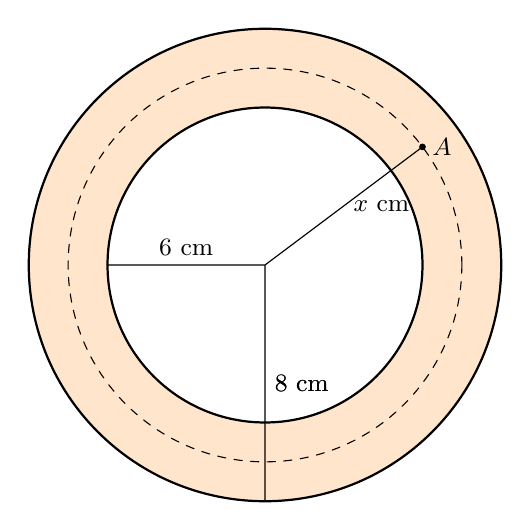
\begin{tikzpicture}[smooth, line cap=round, line join=round,font=\small,scale=1]
			\fill[orange!20] (0,0) circle (3 cm);
			\fill[white] (0,0) circle (2 cm);
			\draw[thick] 
			(0,0) circle (2 cm)
			(0,0) circle (3 cm)
			;
			\draw[dashed] (0,0) circle (2.5 cm);
			\draw (0,0)--node[midway, above]{$6$ cm}(-2,0) (0,0)--node[midway,right]{$8$ cm}(0,-3) (0,0)--node[midway,right]{$8$ cm}(0,-3) (0,0)--node[midway,right]{$x$ cm}(2,1.5) 
			;
			\draw[fill] (2,1.5) circle (1pt) node[right]{$A$};
		\end{tikzpicture}
	\end{center}
	Tìm nhiệt độ mặt ngoài của ống (làm tròn kết quả đến hàng phần chục).
	\loigiai{
			\begin{center}
			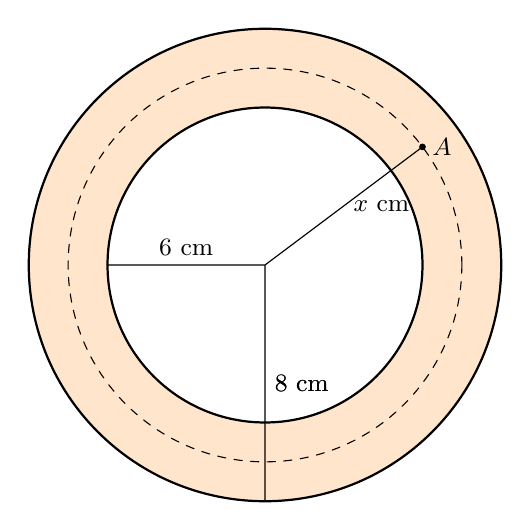
\begin{tikzpicture}[smooth, line cap=round, line join=round,font=\small,scale=1]
				\fill[orange!20] (0,0) circle (3 cm);
				\fill[white] (0,0) circle (2 cm);
				\draw[thick] 
				(0,0) circle (2 cm)
				(0,0) circle (3 cm)
				;
				\draw[dashed] (0,0) circle (2.5 cm);
				\draw (0,0)--node[midway, above]{$6$ cm}(-2,0) (0,0)--node[midway,right]{$8$ cm}(0,-3) (0,0)--node[midway,right]{$8$ cm}(0,-3) (0,0)--node[midway,right]{$x$ cm}(2,1.5) 
				;
				\draw[fill] (2,1.5) circle (1pt) node[right]{$A$};
			\end{tikzpicture}
		\end{center}
		Hàm nhiệt độ $T(x)$ trên thành ống là một nguyên hàm của hàm số $T^{\prime}(x)=-\dfrac{30}{x}$ nên ta có 
		\begin{center}
			$T(x)=-30\ln x+C$ với $6\leq x \leq 8$.
		\end{center}
	Khí bên trong ống được duy trì ở $150\,^\circ\mathrm{C}$ suy ra 
	\begin{center}
		$T(6)=150 \Leftrightarrow -30\ln6+C=150 \Leftrightarrow C=30\ln 6+150$.
	\end{center}
	Suy ra $T(x)=-30\ln x+30\ln6+150$.\\
	Nhiệt độ mặt ngoài của ống là $F(8)=-30\ln 8+30\ln6+150\approx 141{,}4\,^\circ\mathrm{C}$.
}
\end{ex}
\begin{ex}%[2D4V2-2]%%[Dự án D đợt 4 - Nguyễn Hoàng Anh]%[Đề ôn tập Chương IV - Khối 12 - Đề số 3]
	Cho hàm số $f(x)$ liên tục trên $\mathbb{R}$, biết $f(x)=16x^3-15x^2+2x\displaystyle\int\limits_1^2f(t)\mathrm{\,d}t-21$. Giá trị của $f(2)$ bằng bao nhiêu?
	\loigiai{Đặt $m=\displaystyle\int\limits_1^2f(t)\mathrm{\,d}t$.\\
		Từ giả thiết ta có $f(x)=16x^3-15x^2+2mx-21$. Do đó nên
		\begin{eqnarray*}
			&&m=\displaystyle\int\limits_1^2\left(16t^3-15t^2+2mt-21\right)\mathrm{\,d}t\\
			&\Leftrightarrow&m=\left(4t^4-5t^3+mt^2-21t\right)\bigg|_1^2\Leftrightarrow m=-2.
		\end{eqnarray*}
		Thay $m=-2$ vào hàm số ta có $f(x)=16x^3-15x^2-4x-21$, suy ra $f(2)=39$.}
\end{ex}
\begin{ex}%[2D4V3-2]%[Dự án D đợt 4 - Nguyễn Hoàng Anh]%[Đề ôn tập Chương IV - Khối 12 - Đề số 3]
	Một họa sĩ thiết kế logo hình con cá cho một doanh nghiệp kinh doanh hải sản. Logo là hình phẳng giới hạn bởi hai parabol với các kích thước được cho trong hình vẽ sau (đơn vị trên mỗi trục tọa độ là dm).
\begin{center}
	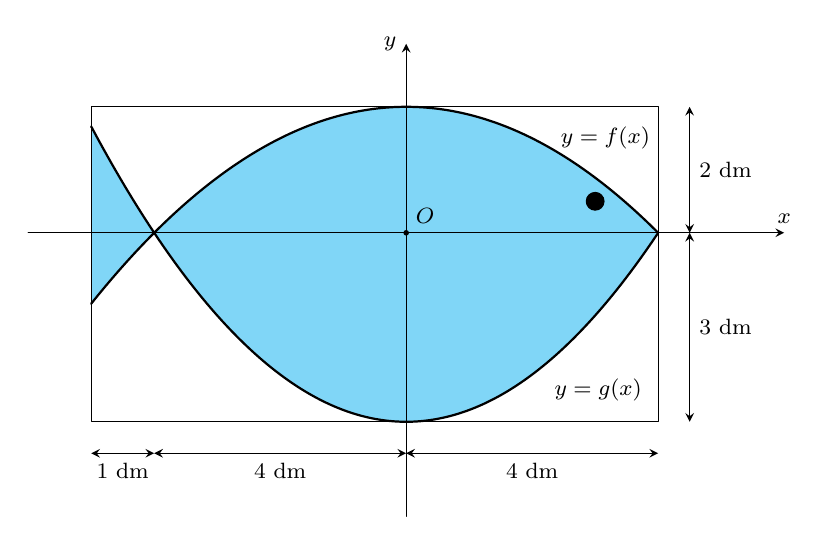
\begin{tikzpicture}[scale=0.8,>=stealth, line join=round, line cap=round,font=\footnotesize]
		\def\xmin{-6} \def\xmax{6}
		\def\ymin{-4.5} \def\ymax{3} 
		%\draw[color=gray!50,dashed] (\xmin,\ymin) grid (\xmax,\ymax); 
		% Tô màu vùng giữa hai đồ thị
		\fill[cyan!50] 
		plot[domain=-5:4, samples=300] (\x,{(-1/8)*(\x)^2+2})
		-- plot[domain=4:-5, samples=300] (\x,{(3/16)*(\x)^2-3})
		-- cycle;
		\draw[->] (\xmin,0)--(\xmax,0) node [above]{$x$};
		\draw[->] (0,\ymin)--(0,\ymax) node [left]{$y$};
		\draw[fill] (0,0 )circle (1pt) node[above right] {$O$};
		\draw[thick,samples=300] plot[domain=-5:4](\x,{(-1/8)*(\x)^2+2});
		\draw[thick,samples=300] plot[domain=-5:4](\x,{(3/16)*(\x)^2-3});
		\draw (-5,-3) rectangle (4,2);
		\draw[fill] (3,.5) circle (4pt);
		\draw[<->] (4.5,0) -- (4.5,2) node[midway,right] {$2$ dm};
		\draw[<->] (4.5,0) -- (4.5,-3) node[midway,right] {$3$ dm};
		\draw[<->] (0,-3.5) -- (4,-3.5) node[midway,below] {$4$ dm};
		\draw[<->] (0,-3.5) -- (-4,-3.5) node[midway,below] {$4$ dm};
		\draw[<->] (-5,-3.5) -- (-4,-3.5) node[midway,below] {$1$ dm};
		\path 
		(2.3,1.5) node[right]{$y=f(x)$}
		(2.2,-2.5) node[right]{$y=g(x)$}
		;
	\end{tikzpicture}
\end{center}
Tính diện tích của logo.
\loigiai{
\begin{center}
	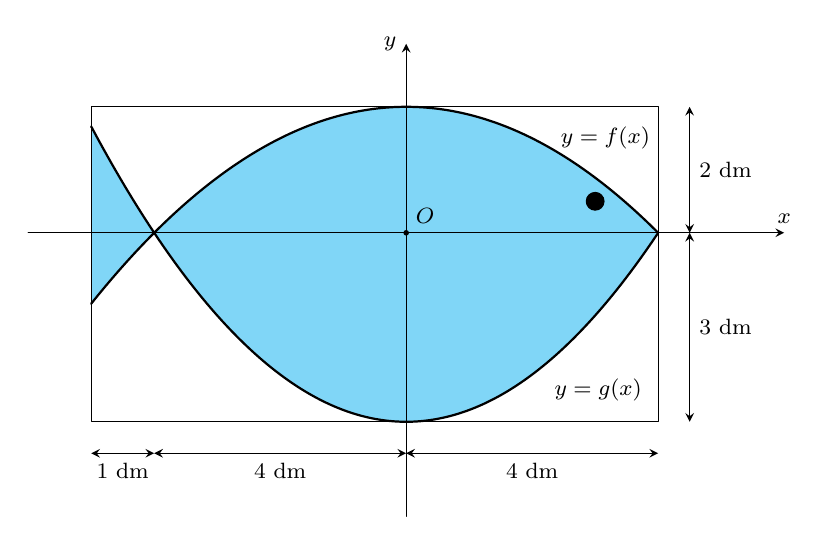
\begin{tikzpicture}[scale=0.8,>=stealth, line join=round, line cap=round,font=\footnotesize]
		\def\xmin{-6} \def\xmax{6}
		\def\ymin{-4.5} \def\ymax{3} 
		%\draw[color=gray!50,dashed] (\xmin,\ymin) grid (\xmax,\ymax); 
		% Tô màu vùng giữa hai đồ thị
		\fill[cyan!50] 
		plot[domain=-5:4, samples=300] (\x,{(-1/8)*(\x)^2+2})
		-- plot[domain=4:-5, samples=300] (\x,{(3/16)*(\x)^2-3})
		-- cycle;
		\draw[->] (\xmin,0)--(\xmax,0) node [above]{$x$};
		\draw[->] (0,\ymin)--(0,\ymax) node [left]{$y$};
		\draw[fill] (0,0 )circle (1pt) node[above right] {$O$};
		\draw[thick,samples=300] plot[domain=-5:4](\x,{(-1/8)*(\x)^2+2});
		\draw[thick,samples=300] plot[domain=-5:4](\x,{(3/16)*(\x)^2-3});
		\draw (-5,-3) rectangle (4,2);
		\draw[fill] (3,.5) circle (4pt);
		\draw[<->] (4.5,0) -- (4.5,2) node[midway,right] {$2$ dm};
		\draw[<->] (4.5,0) -- (4.5,-3) node[midway,right] {$3$ dm};
		\draw[<->] (0,-3.5) -- (4,-3.5) node[midway,below] {$4$ dm};
		\draw[<->] (0,-3.5) -- (-4,-3.5) node[midway,below] {$4$ dm};
		\draw[<->] (-5,-3.5) -- (-4,-3.5) node[midway,below] {$1$ dm};
		\path 
		(2.3,1.5) node[right]{$y=f(x)$}
		(2.2,-2.5) node[right]{$y=g(x)$}
		;
	\end{tikzpicture}
\end{center}
Giả sử $f(x)=ax^2+bx+c$ ($a \neq 0$).\\
Theo giả thiết ta có parabol $y=f(x)$ đi qua các điểm $(4; 0)$, $(-4; 0)$ và $(0; 2)$ nên ta có hệ phương trình
\begin{center}
	$\heva{&16a+4b+c=0\\&16a-4b+c=0\\&c=2} \Leftrightarrow \heva{&a=-\dfrac{1}{8}\\&b=0\\&c=2.}$
\end{center}
Vậy $f(x)=-\dfrac{1}{8}x^2+2$.\\
Giả sử $g(x)=mx^2+nx+p$ ($m\neq 0$).\\
Parabol $y=g(x)$ đi qua các điểm $(4;0)$, $(-4;0)$ và $(0;-3)$ nên ta có hệ phương trình
\begin{center}
	$\heva{&16m+4n+p=0\\&16m-4n+p=0\\&p=-3} \Leftrightarrow \heva{&m=\dfrac{3}{16}\\&n=0\\&p=-3.}$
\end{center} 
Do đó $g(x)=\dfrac{3}{16}x^2-3$.\\
Vì logo là hình phẳng giới hạn bởi hai parabol $y=f(x)$, $y=g(x)$, đường thẳng $x=-5$ và $x=4$ nên diện tích của logo là
\begin{eqnarray*}
	S&=&\displaystyle\int\limits_{-5}^{4} |f(x)-g(x)|\mathrm{\,d}x\\
	&=&\displaystyle\int\limits_{-5}^{-4}\left[g(x)-f(x)\right]\mathrm{\,d}x+\displaystyle\int\limits_{-4}^{4}\left[g(x)-f(x)\right]\mathrm{\,d}x\\
	&=&\displaystyle\int\limits_{-5}^{-4}\left[\dfrac{5}{16}x^2-5\right]\mathrm{\,d}x+\displaystyle\int\limits_{-4}^{4}\left[-\dfrac{5}{16}x^2+5\right]\mathrm{\,d}x\\
	&=&\dfrac{65}{48}+\dfrac{80}{3}\\
	&=&\dfrac{1345}{48}.
\end{eqnarray*}
}
\end{ex}